\chapter{ResNet Initialization and Landscape Analysis}

\section{Reviewing}
\begin{itemize}
\item
Three major tricks for State-of-The-art~(SoTa) Deep Learning Training:
\begin{itemize}
\item
\emph{Initialization};
\item
\emph{Batch Normalization}~(BN);
\item
\emph{ResNet} (or other architectures).
\end{itemize}
\item
Key ideas of Batch Normalization:
\begin{itemize}
\item
Motivation: Reduce condition number by normalization.
\item
Treat Normalization as $\phi$, a non-linear transformation.
\end{itemize}
\item
Error Decomposition~(\emph{An} perspective from Prof. Ruoyu Sun):
\[
\text{Testing Error}=\left\{
\begin{aligned}
&\text{Representation Error}\\
&\text{Optimization Error}
\end{aligned}
\right.
\]
\[
\text{Optimization Error}=\left\{
\begin{aligned}
\text{Finite-time Error}\\
\text{$\infty$-time Error}
\end{aligned}
\right.
\]
\item
How to train a 10000-layer neural network with only one trick ``\emph{initilization}''?
\begin{itemize}
\item
Special Orthogonal Initial point (\text{DeltaOrthogonal});
\item
Based on the idea of Dynamical Isometry.
\end{itemize}
\end{itemize}
\section{Initialization for ResNet}
The architecture for classic ResNet is presented below:
\begin{figure}[H]
\centering
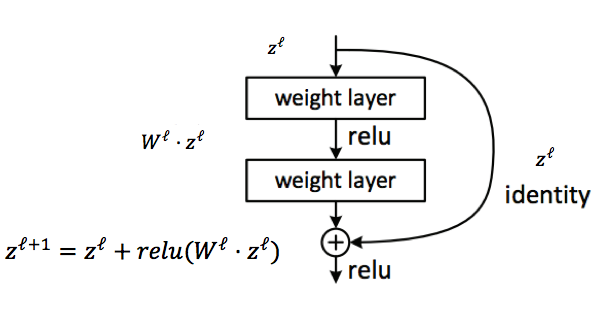
\includegraphics[width=0.8\textwidth]{Fifth_lecture/f_1}
\caption{ResNet framework with Relu activation}
\end{figure}
How to initialize the ResNet architecture? Can we follow the previous knowleage for handling FNN?
Let's give some analysis by first considering the simple linear network~(with the same width).
\begin{example}
Let's consider the $L$-layer linear network with the same width $d$, i.e., the nonlinear activation is an identity operator. 
As a result, the output-input function is expressed as:
\[
y = (I+W^L)\cdots(I+W^1)x,\quad\text{where }W^{\ell}
\in\mathbb{R}^{d\times d}
\]
By the Lecture~2 knowledge, we know that Xavier initialization works for fully connected linear neural networks. Now we perform the simulation of Xavier initialization for ResNet.
The matlab code for the toy example where $L=10$, $d=100$, and input $x$ is all-one vector, is presented below.
\clearpage
\begin{verbatim}
clear;
L = 10;
d = 100;		% dimension for weight matrix W
maxit = 10;	% maximum iteration number	

x = ones(d,1);  norm0 = norm(x);
for i = 1:maxit
    for l = 1:L
        W = randn(d,d)/sqrt(d);
        x = W*x + x;
    end
    rato = norm(x)/norm0
end
\end{verbatim}
Unfortunately, we find that $\|y\|/\|x\|\approx10^{14}$ in this case.
Now the question is the following:
\begin{enumerate}
\item
Why does \citep{He2016res} succeed?

It seems that combining the trick \emph{Batch Normalization} saves him
\item
Why does our simulation fail?

In previous toy example, Xavier initialization works when the output in each layer is the multiplication of the input with a Gaussian matrix, but in our example, 
$(I+W^{\ell})$ is not Gaussian.
\end{enumerate}
Therefore, we need to re-derive the whole \emph{initialization theory} for ResNet, i.e., 
for what kind of $W^{\ell}$, we have $\|y\|/\|x\|\approx\mathcal{O}(1)$?
\begin{enumerate}
\item
Choose $W^{\ell}=\mathcal{N}(0,1/d)-I$, then the original case for linear FNN is recovered, but
we no longer enjoy the advantage of the new architecture.
\item
Consider the case where $d=1$ first, i.e., the output-input function is expressed as
\[
y =(1+w^L)\cdots(1+w^1)x
\]
It's feasible to choose $w^{\ell}=0$ for all $\ell$, but it does not have much representation power, since any point near this initial point will be strongly attracted to it.\footnote{
The formal definition of the strong attraction is presented in the paper \citep{Zhang2000}.
}
It's reasonable to assume that $w^{\ell}$ follows Gaussian distribution, i.e., 
$w^{\ell} = \mathcal{N}(0,\cdot c)$. The question turns to the choice of $c$.
In this case, 
\[
\mathbb{E}[\|y\|^2] = (1+c)^L\|x\|^2
\]
Therefore, we should choose $c=\frac{1}{L}$, which implies $\mathbb{E}[\|y\|^2]=\mathcal{O}(\|x\|^2)$.
\end{enumerate}
For more general $d$, we should make $W^{\ell}_{i,j}=\mathcal{N}(0,\frac{1}{d}\cdot\frac{1}{L})$. The proof outline is as follows:
\begin{itemize}
\item
Consider how the term $\mathbb{E}[\|y\|^2]$ scales with $\|x\|^2$.
Observe that
\begin{align*}
\mathbb{E}[\|z^{\ell}\|^2\mid z^{\ell-1}] = (z^{\ell-1})\trans\bigg[\mathbb{E}(I+W^{\ell})^2\bigg](z^{\ell-1})
\end{align*}
\item
It's easy to show that when $W^{\ell}_{i,j}=\mathcal{N}(0,\frac{1}{d}\cdot\frac{1}{L})$,
\[
\mathbb{E}(I+W)^2 = \mathbb{E}(I+2W+W^2)=I+\mathbb{E}W^2=(1+1/L)I.
\]
\item
Therefore,
\[
\mathbb{E}[\|y\|^2] = (1+1/L)^LI\cdot\|x\|^2=\mathcal{O}(\|x\|^2).
\]
\end{itemize}
\end{example}
\paragraph{Bibilogrphy}
In practice, people notice that ResNet performs much better than standard architectures
when networks are very deep. The paper \citep{Balduzzi2017} gives (partial) explanations for this phenomenon, and claims that one reason is that the gradients in ResNet (with BN) are far more resistant to shattering, which decays sublinearly.
Then this paper proposes a new initialization scheme accordingly, which outperforms the classic He-initialization for standard architectures.

\paragraph{Scaling of the Residuals}
The formal analysis in the paper \citep{Balduzzi2017} is as follows.
Consider a (variant of)~ResNet\footnote{There are several variants of classic ResNet.} framework for Batch Normalization Disabled case:
\[
z^{\ell+1} = \alpha(z^{\ell}+\beta\cdot W^{\ell}\cdot\text{relu}(z^{\ell-1}))
\]
where $\alpha$ and $\beta$ are rescaling factors.
\begin{enumerate}
\item
With classic initilization without batch normalization trick, set $\alpha=\beta=1$, then the variance of the gradient at $z^{\ell}[i]$ is $2^L$.
\item
$\alpha$-scaling: A solution to the exploding variance of resnets is to rescale
layers $\alpha=1/\sqrt{2}$, then $\text{Var}(z^{\ell}[i])=1$.
\item
$\beta$-scaling:
In practice, $\alpha$-rescaling is not used. Instead, combining the bacth normalization trick and $\beta$-scaling\footnote{It's suggested in \citep{Szegedy2016Inceptionv4IA} that $\beta\in[0.1,0.3]$} gives $\text{Var}(z^{\ell}[i])=\beta^2(L-1)+1$.
Furthermore, when $\beta=1/\sqrt{L-1}$, we see that the variance keeps constant:
\[
\text{Var}(z^{\ell}[i])\equiv2.
\]
\end{enumerate}
\paragraph{Is normalization fundamental?}
It's believed that normalization trick is fundamental in state-of-the-art training. The paper \citep{zhang2018residual} challenges this belief by proposing \emph{fixed-update initialization} scheme on \emph{ResNet} to achieve state-of-the-art performance in image classification and machine translation.
This initialization is motivated by solving the gradient explosion/vanishing problem
at the beginning of training via properly rescaling a standard initialization.
This is the only work that achieves such good results without the normalization method


This work is amazing for two reasons:
\begin{enumerate}
\item
Batch Normalization can be annoying, since its practical implementation can have many bugs, especially for ResNet.
\item
It shows the importance of basic logic, i.e., the combination of previous work could have gained more advantages.
The paper \citep{Glorot10understandingthe} first proposes Xavier-initialization; and the same authors propose Relu function in \citep{glorot2011relu}. 
Combining these two tricks, the Kaiming initialization is proposed in \citep{DDR2919332}; and the same authors propose ResNet in \citep{He2016res}.
Moreover, this paper proposes the Fixup initialization by combining these two tricks that enjoy more advantages.
\end{enumerate}

The theme of this course so far: discussion on how the theory shaped the current practice.

\section{Landscape of Neural-Nets}
\paragraph{Motivation}
We are interested in when and why the non-convexity is not a big issue for the training of neural-nets. To answer this question, recall that the Optimization Error is decomposed into two kinds of errors:
\[
\mbox{Optimization Error}\left\{
\begin{aligned}
&\mbox{finite-time error}\\
&\mbox{$\infty$-time error}
\end{aligned}
\right.
\]
It's believed that the major issue is due to the $\infty$-time error, since in practice most algorithms do converge in a reasonable time.
The $\infty$-time error is about the optimality gap between the global minima and the local minima that the algorithm has converged, which is related to the landscape of the loss function for the training of neural-nets.
This lecture will talk about both positive and negative results about the landscape of the loss function.
%\begin{enumerate}
%\item
%Negative Results:
% (due to landscape)
%
%\item
%Positive Results:
%
%\item
%Experimental Findings:
%\end{enumerate}

\subsection{Positive Result: Linear Network has nice landscape}
Consider the loss function for linear neural network with depth $L$:
\[
F(\theta) = \|y - W^L\phi(W^{L-1}(\phi(\cdots W^1x)))\|^2
\]
The non-convexity of this loss function comes from the multi-layer and the non-linear activation.
The case for $L=2$ reduces to the Matrix Factorization problem:
\[
F(\theta) = \|Y - W^2W^1x\|_F^2.
\]
The landscape for matrix factorization is well-studied:

\paragraph{Scalar Case Analysis}
The loss function for the scalar case is given by:
\[
F(u,v) = (1-uv)^2,\qquad u,v\in\mathbb{R}.
\]
The 3-D plot for this loss function is in Fig.~\ref{fig:5:2}.
\begin{figure}[H]
\centering
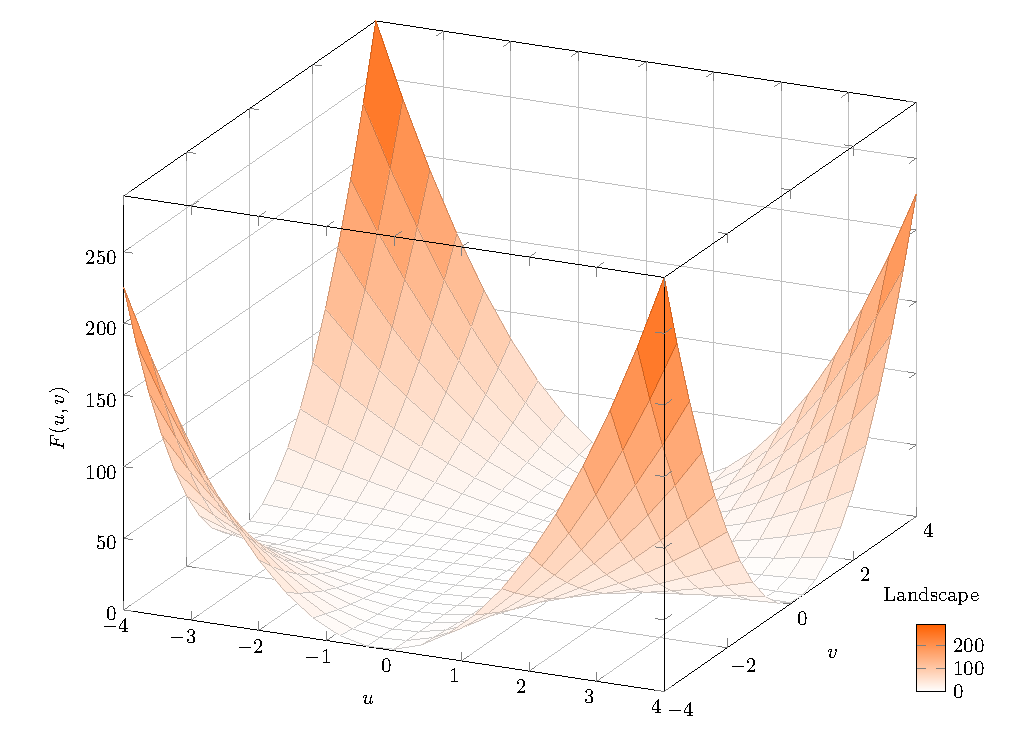
\includegraphics[width=0.8\textwidth]{Fifth_lecture/f_2.pdf}
\caption{$3$-D plot for the loss function $F(u,v) = (1-uv)^2$}
\label{fig:5:2}
\end{figure}
From the landscape we can see that every local minima is a global-minima, i.e., there is no bad local minima.
We give a proof for this claim:
\begin{enumerate}
\item
Step 1: By taking gradient equal to zero, we find stationary points must satisfy
\[
\text{either $uv=1$ or $u=v=0$}
\]
\item
Step 2: It suffices to show that $(u,v) = (0,0)$ is not a local-minima. Note that 
\[
F(\epsilon_1,\epsilon_2) = (\epsilon_1\epsilon_2-1)^2<1
\]
When $(\epsilon_1,\epsilon_2)>0$ are sufficiently small, we find the function value decreases, i.e., $(0,0)$ is not a local-minima.
\end{enumerate}
\begin{remark}
However, starting from $(u,v)=(0,0)$, the gradient descent gets stuck.
Is this finding bad enough? 
Actually not. The paper~\citep{pmlr-v49-lee16} shows that gradient descent, if converges, it only converges to a local minimizer, almost surely with random initialization.
The recent trend for non-convex optimization is not satisfied with the convergence to first order stationary point\footnote{$\epsilon$-First order stationary point~(FOSP) means $\|\nabla f(x)\|\le\epsilon$}, but the convergence to second order stationary point.\footnote{Second order stationary point~(SOSP) means $\nabla f(x)=0$ and $\nabla^2f(x)\succeq0$.}
The reason is that empirically second order stationary point is as good as global minima.
The tutorial \citep{ISIT2019} in ISIT2019
gives summarization on the recent progress in non-convex optimization, which is highly recommended to read.
\end{remark}

However, for people working on optimization, focusing on second order stationary point is not good enough, since high-order saddle points do exist for deep neural-nets.
Now let's focus on the second order stationary point only.

\begin{proposition}
Consider the function $F(u) = \|M - uu\trans\|_F^2$, where $M$ is PSD, any SOSP of this function is global-minima.
\end{proposition}
\begin{proof}
\begin{enumerate}
\item
Step 1: Check the gradient:
\[
\nabla_u F = 4(M - uu\trans)u=0\implies Mu = (u\trans u)u
\]
Therefore, if $u$ is SOSP, then $(\|u\|^2,u)$ is an eigen-pair of $M$.
\item
Check the Hessian of the SOSP $u$:
\[
\nabla^2F(u)=4(uu\trans + \|u\|^2I-M)\succeq0.
\]
\end{enumerate}
Combining these steps, we can show that $\|u\|^2=\lambda_{\max}(M)$, i.e., $u$ is a global-minima.
\end{proof}


\paragraph{Re-thinking Convexity}
From this proof we can partially answer why many people work on convex optimization, and why non-convex optimization is not scary:
\begin{enumerate}
\item
By sub-gradient inequality, we can show that FOSP together with convexity implies global-minima.
Therefore, it suffices to design algorithms searching for FOSP.
\item
Define $G\triangleq\{\text{SOSP implies global-minima}\}$. We find many instances belong to the set $G$:
\[
\{\text{convex problems}\}\subseteq G,\qquad
\{\min_{u}\|M - uu\trans\|_F^2\}\subseteq G.
\] 
Therefore, for non-convex problems belonging to the set $G$, it suffices to design algorithms searching for SOSP.
\end{enumerate}

\paragraph{Bibliography}
The paper \citep{BALDI198953} shows that any SOSP for the $2$-layer linear network quadratic loss function is global-minima under mild conditions;
the paper \citep{NIPS2016_6112} shows that any SOSP for the deep linear network quadratic loss function is global-minima under mild conditions.
There are many later works extending to other loss functions.
Up to now, we find that multi-layer may not be an issue.

\subsection{Negative Result: Nonlinearity doesn't necessarily imply Global-optimality for SOSP}
Now consider the non-linear activation. For the $1$-dimension case, suppose the loss function $F(w) = (y - \phi(wx))^2$. W.l.o.g., $x=y=1$, which follows that
\[
F(w) = (1-\phi(w))^2.
\]
We are interested in whether all SOSP are global-minimas.
\paragraph{Relu Activation}Now we draw the landscape of $F(w)$ if $\phi(w)=\max\{w,0\}$:
\begin{figure}[H]
\centering
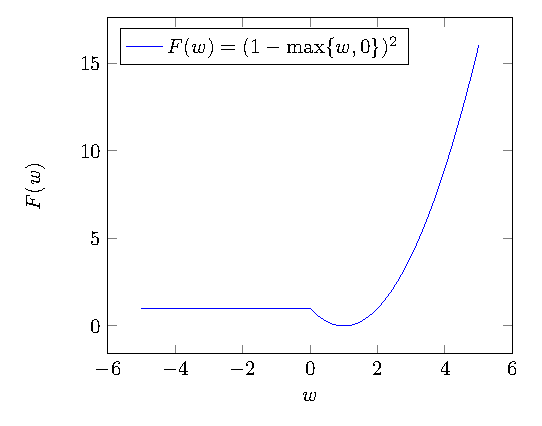
\includegraphics[width=0.6\textwidth]{Fifth_lecture/f_3.pdf}
\caption{$2$-D plot for the loss function $F(w) = (1-w_+)^2$}
\label{fig:5:3}
\end{figure}
We find that for $w<0$, $w$ is still a SOSP, but no longer a global-minima.
Let's try other kinds of activation functions.
\begin{itemize}
\item
When $\phi(w)=w^2$, we find SOSPs are still the global-minima:
\begin{figure}[H]
\centering
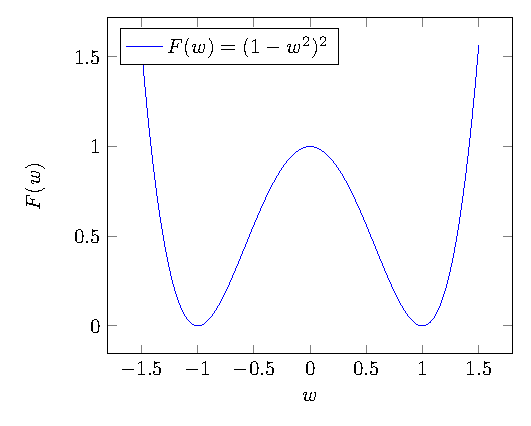
\includegraphics[width=0.6\textwidth]{Fifth_lecture/f_4.pdf}
\caption{$2$-D plot for the loss function $F(w) = (1-w^2)^2$}
\label{fig:5:4}
\end{figure}
\item
When $\phi(w)=\text{sigmoid}(w)=\frac{1}{1+e^{-w}}$, we find SOSP is still the global-minima:
\begin{figure}[H]
\centering
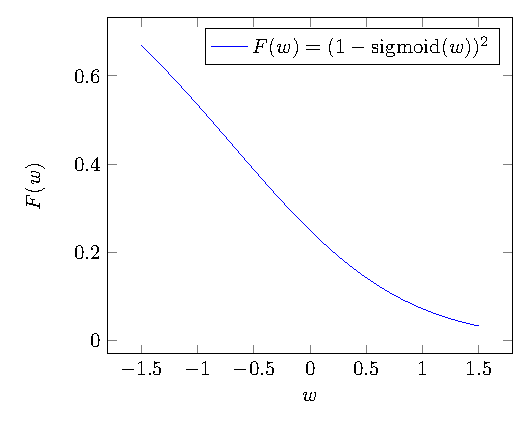
\includegraphics[width=0.6\textwidth]{Fifth_lecture/f_5.pdf}
\caption{$2$-D plot for the loss function $F(w) = (1-\text{sigmoid}(w))^2$}
\label{fig:5:5}
\end{figure}
\end{itemize}
Therefore, we conclude that the landscape of loss function is fine for most non-linear activations.
but ReLu is not good in terms of landscape.
Prof. Ruoyu Sun suggests that we can try Leaky Relu or Softplw if Relu fails (e.g., for GAN training).

In the next lecture we will try the sum of loss functions, i.e., 
\[
F(w) = (y_1-\phi(w)x_1)^2+(y_2-\phi(w)x_2)^2.
\]
The question is that if two functions both have good landscapes, does the summation still have a good landscape?




